\section*{Ergebnisse und Fatzit}


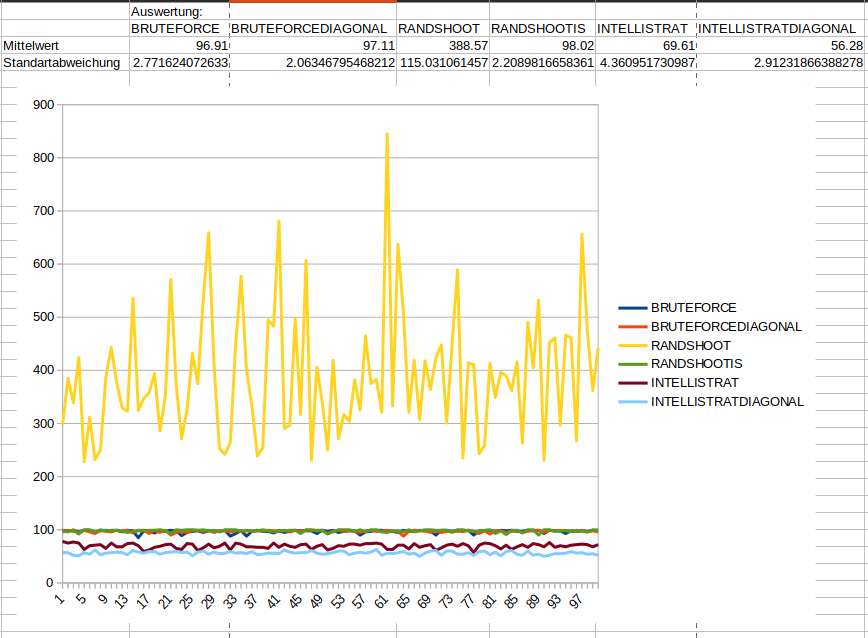
\includegraphics[scale=0.5]{Screenshot from 2022-02-08 08-28-03.png}
Die Ergenisse darstellen und auswerten (erklären wie wir auf die Ergebnisse gekommen sind Standartabweichung etc.)

Bei den sechs Strategien sind teils erhebliche Unterschiede in der Anzahl der durchschnittlich benötigten Schüsse um ein Spiel zu gewinnen zu erkennen. Die Strategie die die meisten 
Schüsse benötigt ist Randshoot, dies ist zu erwarten da die Strategie auf zufällig ausgewählte Felder schießt, aber nicht speichert welches Feld bereits beschossen wurde. So ist es 
fast unvermeidlich, dass Felder mehrmals beschossen werden. Die Strategie RandshootiS ist eine Erweiterung der Strategie Randshoot, ihre funktion ist identisch nur wurde sie 
erweitert dass bereits beschossene Felder gespeichert werden um so ein mehrmaliges beschießen zu verhindern. Das Ergebniss dieser Erweiterung lässt sich anhand der durchschnittlichen 
Anzahl der Schüsse und der Standartabweichung beobachten, die Anzahl der benötigten Schüsse und der Wert der Standartabweichung sind signifikant gesunken. Die Strategien Bruteforce 
und BruteforceDiagonal weisen eine ähnlich hohe Anzahl von durchschnittlichen Schüssen auf, da ihr Grundprinzip das gleiche ist. Die durchschnittliche Anzahl von Schüssen im Bereich 
von 97 kommt dadurch zu stande, da beide Startegien jedes Feld nacheinander beschießen und es nur 100 Felder maximal gibt. Die Strategien Intellistrat und IntellistratDiagonal sind \
die beiden effizientesten Strategien. Intellistrat macht sich die Funktion Neigbour zu nutze, welche bei einem Treffer geziehlt nach dem Schiff sucht und es sofort zerstört. 
IntellistratDiagonal nutzt diese Funktion auch, jedoch durch das Diagonale abgehen der Felder kann jeweils ein Feld horizontal ausgelassen werden und so ein Spiel in noch weniger 
Schritten gewonnen werden.

Die Random und Bruteforce Strategien weisen eine einfache Code-Strucktur auf benötigen jedoch mehr Schüsse, RandShoot ist ein Extrembeispiel, während die Intellistrat Strategien 
komplexere Methoden benötigen, jedoch eiffizienter und schneller gewinnen.